\documentclass[12pt,letterpaper]{article}

\usepackage{graphicx,
			amssymb,
			amsmath,
			titlesec,
			lipsum,
			setspace,
			lastpage,
			fancyhdr,
			tikz,
			titling}
\usepackage{tkz-euclide}
\usepackage{setspace}

\usetkzobj{all}
\usetikzlibrary{shapes,arrows}
\tikzstyle{block} = [rectangle, draw, fill=blue!20,
text centered, rounded corners, minimum height=2em]

\tikzstyle{line} = [draw, -latex']
\newenvironment{my_enumerate}{
	\begin{enumerate}
	\setlength{\itemsep}{1pt}
	\setlength{\parskip}{0pt}
	\setlength{\parsep}{0pt}}{\end{enumerate}
}

%% Figure caption formatting
\usepackage[labelfont=it,textfont=it,labelsep=period]{caption}
\usepackage[labelfont=it,textfont=it,labelsep=period]{subcaption}

%% Overall margins
\usepackage[margin=1in]{geometry}

%% Footer formatting
\fancyhf{}
\renewcommand{\headrulewidth}{0pt}
\pagestyle{fancy}
\cfoot{\textbf{\textsf{Page\ \thepage\ of \pageref{LastPage}}}}

%% Author list formatting
\newenvironment{nscenter}
 {\parskip=0pt\par\nopagebreak\centering}
 {\par\noindent\ignorespacesafterend}

\newcommand{\affiliatedauthor}[2]{
\begin{nscenter}
	#1 \\ \textit{#2}
\end{nscenter}
}

%% Abstract formatting
\renewcommand{\abstractname}{ABSTRACT}

\renewenvironment{abstract}
 {\vspace{-0.5ex}
	\small
	\begin{center}
		\bfseries \abstractname\vspace{-4ex}\vspace{0pt}
	\end{center}
	\list{}{
		\setlength{\leftmargin}{0.5in}
		\setlength{\rightmargin}{\leftmargin}
	}
	\item\relax}
 {\endlist}

%% Section header formatting
\renewcommand\thesection{}
\renewcommand\thesubsection{}
\renewcommand\thesubsubsection{}
\titleformat{\section}{\normalfont\bfseries}{\thesection}{1em}{}
\titleformat{\subsection}{\normalfont\bfseries}{\thesubsection}{1em}{}
\titleformat{\subsubsection}{\normalfont\itshape}{\thesubsubsection}{1em}{}
\titlespacing*{\section}{0pt}{2ex}{-1.5ex}
\titlespacing*{\subsection}{0pt}{2ex}{-1.5ex}
\titlespacing*{\subsubsection}{0pt}{2ex}{-1.5ex}

%% Paragraph formatting (changing this messes with literally everything)
\setlength{\parindent}{0pt}
\setlength{\parskip}{2ex}
\newcommand\tab[1][1cm]{\hspace*{#1}}

\title{Intelligent Quadcopter for IARC 2018}

\begin{document}

\begin{center}
	\textbf{\LARGE{\thetitle}}
\end{center}

%%%%%%%%%%%% SET AUTHOR NAMES AND AFFILIATIONS %%%%%%%%%%%%
\affiliatedauthor{Noel Brownback}{The University of Texas at Austin}
\affiliatedauthor{Anthony Carreon}{The University of Texas at Austin}
\affiliatedauthor{Shayer Hassan}{The University of Texas at Austin}
\affiliatedauthor{Eric Johnson}{The University of Texas at Austin}
\affiliatedauthor{Colin Lewis}{The University of Texas at Austin}
\affiliatedauthor{Mark Loveland}{The University of Texas at Austin}
\affiliatedauthor{Umer Salman}{The University of Texas at Austin}
\affiliatedauthor{Ethan Starr}{The University of Texas at Austin}
%%%%%%%%%%%%%%%%%%%%%%%%%%%%%%%%%%%%%%%%%%%%%%%%%%%%%%%%%%%


%%%%%%%%%%%%%%%%%%%%%%% ABSTRACT %%%%%%%%%%%%%%%%%%%%%%%
\begin{abstract}
	Texas Aerial Robotics has constructed a custom quadrotor aircraft for the fulfillment of the International Aerial Robotics Competition Mission 7. A combination of lightweight materials and powerful propulsion enables optimizes flight time, while standardized flight control systems supported by a massive community enabled customization and adaptation to the mission at hand. This includes the integration of a multitude of sensors that enhance environmental awareness and allow for the tracking of dynamic entities inherent to the operation using homebrewed algorithms and the significant computing power onboard the aircraft. Safe development has been assured by strategic selection of components, thorough vetting of software in Software in the Loop simulation, and robust testing procedures in secure areas.
\end{abstract}
%%%%%%%%%%%%%%%%%%%%%%%%%%%%%%%%%%%%%%%%%%%%%%%%%%%%%%%%

%%%%%%%%%%%%%%%%%%%%%% MAIN TEXT %%%%%%%%%%%%%%%%%%%%%%

\section*{Introduction}
	Previous aerial robotics missions have always allowed for GPS or set navigation points that allowed for constant locational awareness for the drone. Location data is important to any mission, as telemetry prevents various failures, including complete loss of control for the drone. Thus, Mission 7 requires novel solution to deriving this critical telemetry, as GPS is forbidden. Additionally, the aircraft must be capable of interacting with ground vehicles without being directly informed of their locations, requiring advanced detection and robust hardware designed for repeated contact.

	Texas Aerial Robotics addresses these challenges by utilizing computer vision. Through computer vision the drone has the ability to both understand its location, and also track targets in real time. The drone records the data and position of the objects, simulating those which lie beyond the field of view, which allows for strategic analysis and definition based on estimates of unseen/out of sight targets. Interaction with these objectives is achieved using the carbon fiber bottom plate of the aircraft and perimeter prop guards, a material choice that lends itself to lightweight resiliency.

	\begin{figure}[!htbp]
	\begin{center}
	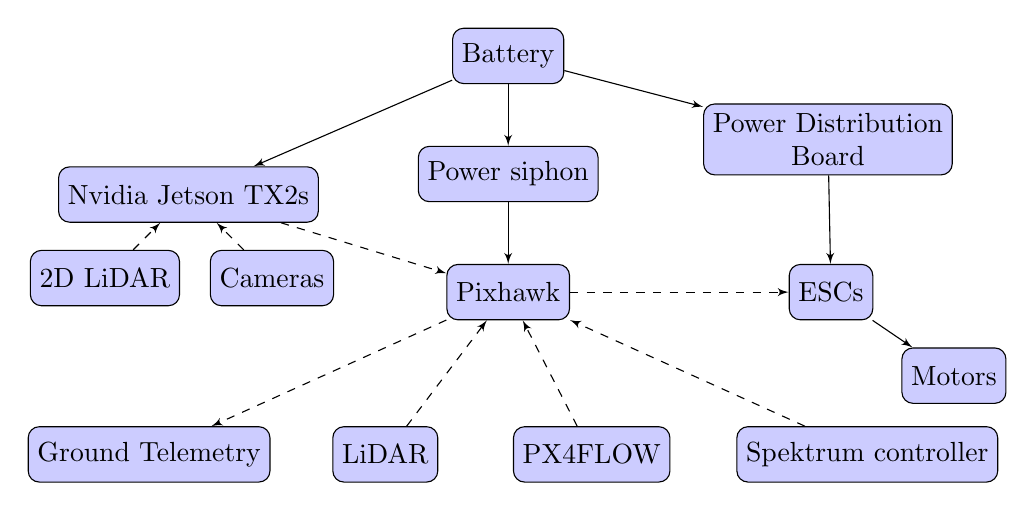
\begin{tikzpicture}[node distance = 1.5cm and 8cm, auto]
		% Place nodes
		\node [block] (battery) {Battery};
		\node [block, below of=battery] (siphon) {Power siphon};
		\node [block, below of=siphon] (Pixhawk) {Pixhawk};
		\node [block, below right of=battery, xshift=3cm, align=center] (PDB) {Power Distribution \\ Board};
		\node [block, below left of=battery, xshift=-3cm, yshift=-.7cm] (Jetson) {Nvidia Jetson TX2s};
		\node [block, right of=Pixhawk, xshift=2.6cm] (ESCs) {ESCs};
		\node [block, below right of=ESCs, xshift=.5cm] (Motors) {Motors};
		\node [block, below right of=Jetson] (Camera) {Cameras};
		\node [block, below left of=Jetson] (2dLidar) {2D LiDAR};
		\node [block, below right of=Pixhawk, yshift=-1cm] (Flow) {PX4FLOW};
		\node [block, below right of=Pixhawk, xshift=3.5cm, yshift=-1cm] (Spektrum) {Spektrum controller};
		\node [block, below left of=Pixhawk, xshift=-.5cm, yshift=-1cm] (LiDAR) {LiDAR};
		\node [block, below left of=Pixhawk, xshift=-3.5cm, yshift=-1cm] (Telemetry) {Ground Telemetry};
		% Draw edges
		\path [line] (battery) -- (siphon);
		\path [line] (siphon) -- (Pixhawk);
		\path [line] (battery) -- (PDB);
		\path [line] (PDB) -- (ESCs);
		\path [line] (battery) -- (Jetson);
		\path [line, dashed] (Camera) -- (Jetson);
		\path [line, dashed] (2dLidar) -- (Jetson);
		\path [line, dashed] (Flow) -- (Pixhawk);
		\path [line, dashed] (Jetson) -- (Pixhawk);
		\path [line, dashed] (LiDAR) -- (Pixhawk);
		\path [line, dashed] (Pixhawk) -- (Telemetry);
		\path [line, dashed] (Spektrum) -- (Pixhawk);
		\path [line, dashed] (Pixhawk) -- (ESCs);
		\path [line] (ESCs) -- (Motors);
	\end{tikzpicture}
	\caption*{Flowchart of quadcopter electronics \\ \tiny *Solid arrows indicate power while dashed lines indicate power+data}
	\end{center}
	\end{figure}

	\subsection*{Yearly Milestones}
	2017 - Have a working bot, with computer vision software in working or nearly working
	2018 - Continue development of computer vision, develop a computational game strategy through creation of simulations of the motion of Roombas, tweak the physique of the drone for better flight control and stability


\section*{Air Vehicle}
	\subsection*{Propulsion and Lift System}
			The vehicle utilizes a x-y axis symmetrical quad-rotor system. This provides a balanced airframe optimized for omni-directional maneuvering. The frame is lifted by four T-Motor U3 KV700 motors. These motors provide 1.8 [kg] of thrust per motor at 100\% throttle when paired with a 4-cell battery and 13 [in] propellers for total 7.2 [kg] of thrust. This is necessary for our 3.15 kg weight to maintain a 2.2 thrust-to-weight ratio ideal for battery life and flight time.

			The propellers used with the motors are 13 [in] long and made of carbon fiber. These T-Motor propellers provide excellent precision, durability, and efficiency. The rotors are placed to counter-rotate for flight stability and to retain a one-to-one ratio of propellers to motors.


	\subsection*{Guidance, Navigation, and Control}
		\subsubsection*{Stability Augmentation System}
			Our system builds off of the robust open source project Arducopter. Arducopter, runs on the Pixhawk, and controls the stability of the drone by taking in data from the IMU, compass, altitude LiDAR and the optical flow sensor. The Arducopter flight stack is maintained by hundreds of developers from around the world and the software is deployed on thousands of commercial and recreational drones. The vast community of developers and users ensures refined controls code with lots of features.


		\subsubsection*{Navigation}
			We have made slight modifications to the Arducopter firmware, which allow us to set the EKF origin. This has been done to allow our drone to navigate in GPS denied environments. For general waypoint navigation, the drone utilizes the Arducopter EKF that takes in data from the IMU, compass, altitude LiDAR and the optical flow sensor. The EKF position is then queried via mavros, so that our strategy code can use our position to make intelligent decisions. In addition, the strategy node takes in data from computer vision and 2D LiDAR. The strategy will determine a waypoint and mode, and the ros controls node will do a sanity check on the waypoint, then publish the waypoint until the drone has reached its destination. Over time, the EKF will have error in comparison to reality. To combat this, the control node will input a correction vector. This correction vector is formed from our computer vision algorithm that recognizes the absolute corners of the grid. This algorithm goes as follows. Gaussian blur, color threshold, erosion, dilation, Canny, Hough, line intersection, and non maximum suppression.

		\begin{figure}[!htbp]
			\begin{center}
				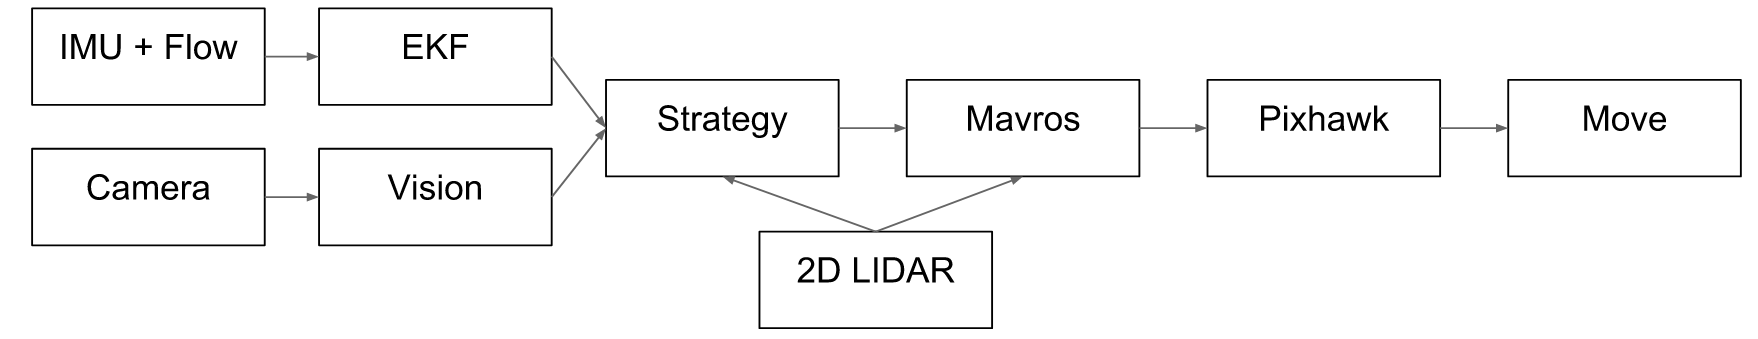
\includegraphics[width=0.75\textwidth]{system}
				\caption*{Overview of control system}
			\end{center}
		\end{figure}

		% \begin{figure}[!htbp]
		% 	\begin{center}
		% 		\begin{tikzpicture}[node distance = 3cm, auto]
		% 			% Place nodes
		% 			\node [block] (IMU) {IMU + Flow};
		% 			\node [block, below of=IMU] (Camera) {Camera};
		% 			\node [block, right of=IMU] (EKF) {EKF};
		% 			\node [block, below of=EKF] (Vision) {Vision};
		% 			\node [block, below right of=EKF] (Strategy) {Strategy};
		% 			\node [block, below right of=Strategy] (2DLiDAR) {2D LiDAR};
		% 			\node [block, right of=Strategy] (mavros) {mavros};
		% 			\node [block, right of=mavros] (Pixhawk) {Pixhawk};
		% 			\node [block, right of=Pixhawk] (Move) {Move};
		% 			% Draw edges
		% 			\path [line] (IMU) -- (EKF);
		% 			\path [line] (Camera) -- (Vision);
		% 			\path [line] (EKF) -- (Strategy);
		% 			\path [line] (Vision) -- (Strategy);
		% 			\path [line] (2DLiDAR) -- (Strategy);
		% 			\path [line] (2DLiDAR) -- (mavros);
		% 			\path [line] (Strategy) -- (mavros);
		% 			\path [line] (mavros) -- (Pixhawk);
		% 			\path [line] (Pixhawk) -- (Move);
		% 		\end{tikzpicture}
		% 		\caption*{Overview of control system}
		% 	\end{center}
		% \end{figure}

		\subsubsection*{Flight Termination System}
			Our drone houses a 40 [A] brushless ESC connected to a RC receiver, which acts as our kill switch. In the event of catastrophic failure the safety operator can send the kill signal, and all power will be cut to the drone's systems.


\section*{Payload}
	The drone has been designed to carry all the necessary GNC sensors, 2D LiDAR, and array of cameras and 3 Nvidia Jetson TX2s. In addition the drone carries a telemetry radio, kill switch, and RC receiver in order to carry out safe flight.
	\subsection*{Sensor Suite}
		\subsubsection*{GNC Sensors}
			The quadcopter uses eight sensors for flight control. The main sensors used for the navigation of the quadcopter are a downwards-facing 1D LiDAR module, a PX4FLOW optical sensor, and the built-in sensors of our flight control board, the Pixhawk 2.

			The 1D LiDAR module used is the LiDAR-lite v3 from Garmin. This one dimensional sensor is directed downwards and provides data that is used to determine altitude. The PX4FLOW sensor measures velocity by comparing frame by frame images and measuring distance travelled and direction. The Pixhawk 2 contains three 3-axis accelerometers, three 3-axis gyroscopes, and two 3-axis compasses. The data from these sensors is used by the Pixhawk onboard system for flight control and the maneuvering of the quadcopter.

		\subsubsection*{Mission Sensors}
			For the goal of completing Mission 7 the drone must be able to detect Roombas and obstacles. The quadcopter is equipped with a single downward facing camera, four outward facing cameras, and a two-dimensional plane LiDAR sensor for obstacle avoidance.
			The singular bottom camera is a Logitech C210 webcam. This webcam is used for Roomba detection and tracking the targeted Roomba for autonomous interaction.For the four peripheral cameras are Logitech 960 C270. These are used to recognize and track the Roombas around the playing field. These five webcams provides enough information allowing the drone to incorporate the recognized Roombas into the strategy of the autonomous system.
			The 2D LiDAR sensor is the SWEEP sensor by Scanse. This is a single LiDAR that rotates to provide a full x-y plane view inline with the z position of the drone for obstacle detection. We chose to use this for obstacle detection rather than four separate LiDARs or webcams to save on computing power.


		\subsection*{Target Identification}
			For target identification, the drone carries four Logitech C270 USB webcams and one Logitech C210 USB webcam. One of the cameras is located at the bottom of the drone and faces straight downward. The other four cameras are mounted on the bottom side of each arm facing outward. All five cameras are mounted for identifying as many target Roombas surrounding the drone as possible in order to send their coordinates to the strategy node.

			There are two main objectives that need to be completed to successfully relay target information to the strategy node. The first objective is to take in the raw video data and detect the target Roombas so that pixel numbers of the centroids of the Roombas in the frame can be sent as output. The second objective is to take the pixel numbers of the centroids of the detected Roombas as input, and then output x and y coordinates relative to the drone using a coordinate transformation and the known height and orientation of the camera with respect to the floor.

			In order to accomplish the first objective, an open source software package developed by Joseph Redmon called YOLO (You Only Look Once) is used. More specifically, the TinyYolo version of YOLO was elected to be used since it is lighter and can obtain higher frame rates. YOLO is a neural network that can identify user-defined objects once it has been trained. After training the neural network by feeding in approximate 2000 photos of the target Roombas (with the Roombas identified manually), YOLO can reliably identify target Roombas in real time. An example is displayed below:

			\begin{figure}[!htbp]
				\begin{center}
					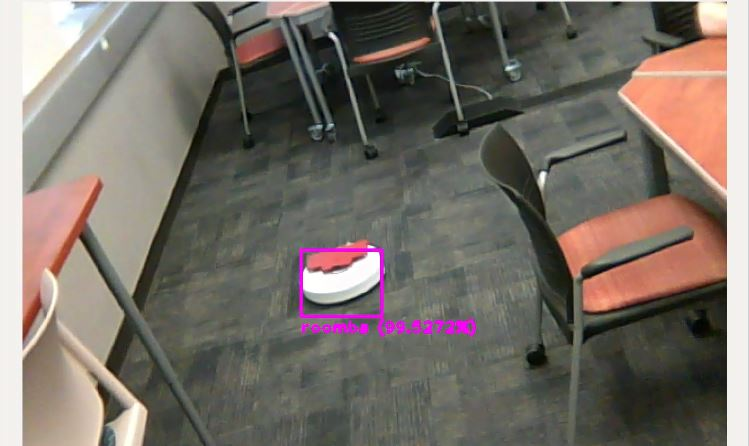
\includegraphics[width=0.75\textwidth]{roomba}
				\end{center}
			\end{figure}

			After YOLO outputs the pixel locations of each identified target Roomba, the final objective is to transform these pixel coordinates into x-y coordinates relative to the drone. In addition to the pixel coordinate (PIX \#), the other knowns are height ($z$), camera rotation angle relative to downward facing ($\theta$), and field of view ($\phi$), as well as total pixels in x and y (PIX\_MAX). Here is a diagram to illustrate these knowns below:

			\begin{tikzpicture}[scale=3]
				\coordinate [label=left:$X$] (X) at (-1.5cm,-1cm);
				\coordinate [label=right:$Y$] (Y) at (1.5cm,-1cm);
				\coordinate [label=above:$Z$] (Z) at (-1.5cm,1cm);
				\coordinate (phi) at (.1cm,-1cm);
				\coordinate (theta) at (-.75cm,-1cm);
				\draw[<->] (Z) -- node[below] {} (X) -- node[right] {} (Y);
				\draw[dashed](Y) -- node[above left] {} (Z);
				\draw[dashed] (Z) -- node[below] {} (phi);
				\draw[dashed] (Z) -- node[below] {} (theta);
				\tkzMarkRightAngle[draw=black](Z,X,Y)
				\tkzDrawPoints[color=black,fill=white](X)
				\tkzMarkAngle[size=1cm,color=cyan](X,Z,phi)
				\tkzMarkAngle[size=1.5cm,color=cyan](theta,Z,Y)
				\tkzLabelAngle[dist=1.6cm](theta,Z,Y){$\phi$}
				\tkzLabelAngle[dist=1.1cm](X,Z,phi){$\theta$}
			\end{tikzpicture}

			\begin{spacing}{.2}
			In order to transform this pixel coordinate into x-y coordinates relative to the drone, a few key assumptions made are that:

				\begin{itemize}
					\item The camera behaves as a pinhole model
					\item Each pixel in the frame takes up an approximately equal fraction of the field of view
				\end{itemize}

			A big pitfall in this model is that no distortion from the camera lens is accounted for; these effects are still being investigated.

				\textbf{Transformation}:

				Pixel given from YOLO: $PIX$

				Pixel number of the center: $PIX\_CTR = \frac{PIX\_MAX}{2}$

				Define $\psi$ as portion of angle from center image to pixel detected:

				\begin{center}
					$\psi = z * abs(\frac{PIX}{PIX\_MAX} * \phi - \frac{\phi}{2})$
				\end{center}

				To find the real coordinate ($REAL$) relative to the drone in the $X$ direction, There are two cases:

						\tab If $PIX$ lies above the center pixel, that is $PIX > PIX\_CTR$, Then:
						\begin{center}
							$REAL = z * tan(\theta + \frac{\psi}{2})$
						\end{center}
						\tab If $PIX$ lies below the center pixel, that is $PIX < PIX\_CTR$, Then:
						\begin{center}
							$REAL = z * tan(\theta - \frac{\psi}{2})$
						\end{center}
				There are two cases to finding the real coordinate ($REAL$) relative to the drone in the $Y$ direction:

						\tab If $PIX$ lies above the center pixel, that is $PIX > PIX\_CTR$
						\begin{center}
							$REAL = z * tan(\theta - \frac{\psi}{2})$
						\end{center}
						\tab If $PIX$ lies below the center pixel, that is $PIX < PIX\_CTR$
						\begin{center}
							$REAL = z * tan(\theta + \frac{\psi}{2})$
						\end{center}
				This is different from the x only because top of frame is $1$ and bottom is $PIX\_MAX$, while in $X$ 'top' of frame is $PIX\_MAX$ and bottom is $1$.
			\end{spacing}

		Once the coordinate X,Y in meters is found relative to the drone, it must be transformed into a coordinate that is in the 'gym reference frame'. The gym reference frame is defined as a right handed coordinate system starting in the bottom left hand corner of the field where the green line meets the outer white line. This transformation is defined as followed.

		\begin{center}
			$yawAngle = currentHeading - GymOffset$
		\end{center}
		\begin{center}
			$roombaPosGym = CR + EKFdronePose + R(3)(YawAngle)*roombaPosDrone$
		\end{center}

		\[
		R(3) =
			\begin{bmatrix}
			cos(yawAngle) & -sin(yawAngle) & 0 \\
			sin(yawAngle) & cos(yawAngle)  & 0 \\
			0 & 0 & 1
			\end{bmatrix}
		\]

		CR is the correction vector formulated from the corner detection vision algorithm. EKFdronePose is the position of the drone queried from the Pixhawk. R(3) is the rotation matrix about the third axis. GymOffset is the direction of the 2 axis defined during the startup sequence before flight. The new coordinate in the gym frame is passed off to the strategy node as data to be acted on.
	\subsection*{Threat Avoidance}
		Our avoidance system takes data from a 2D LiDAR that is used to identify the obstacle Roombas. This data is passed and the Strategy node uses this data to weigh possible movements negatively based on their relative position to the target Roombas. The Control node also will use the data, and in the event an obstacle robot is within 1.5 [m] will issue a waypoint opposite of the minimum vector.

	\subsection*{Communications}
		On the Jetsons, data is passed between software nodes via ROS. Data in between our multiple Jetsons is passed via ros messages through direct ethernet connections. Commands to the flight computer are passed via serial connection with data encoded in MAVLINK messages.


	\subsection*{Power Management System}
		The quadcopter uses a 10000mAh 4S 10C LiPo battery and a 2000mAh 3S 15C LiPo battery for power. The 10000mAh 4S 10C LiPo is used to power our ESCs and Motors. With 4 T-Motor U3 K700 motors running at close to the ideal 50\% throttle, a 4 Cell battery was necessary to reach the 1800 grams of thrust per motor needed for hovering flight. The 2000mAh 3S 15C LiPo will power the flight control board and Jetson compute units.
		\begin{center}
			$T_{min} = \frac{\text{Battery power}(AH) * 60}{\text{Total current drawn by motors}}$
		\end{center}

		Assuming an average throttle of 65\% for maneuvering, we see a 9 A current draw from each motor, and with a 10 Ah battery, that provides us with 16 minutes of flight time with minimal maneuvering and height change. This gives us plenty of headroom for more intense altitude and positioning changes, which will allow us to move more quickly during the competition, a valuable asset with the given time limitation.
		\begin{center}
			Max continuous Amp draw ($A$) = Battery capacity ($Ah$) $*$ Discharge rate ($C$)
		\end{center}

		To save on weight and space, we chose a 10C discharge rate battery, as this is still more than enough to match the maximum continuous current draw of 25 [A] and maximum practical current draw of 19.4 [A] required by the motors. The 10000 [mAh] battery with a 10C discharge rate gives us a maximum continuous current draw of 100 [A], matching the limit of the motors.

		The eCalc online tool was used to validate our calculations, and as seen by the generated graph below, there should be no issue reaching above-10 minute flight times at speeds below 15 [mph]

		\begin{figure}[!htbp]
			\begin{center}
				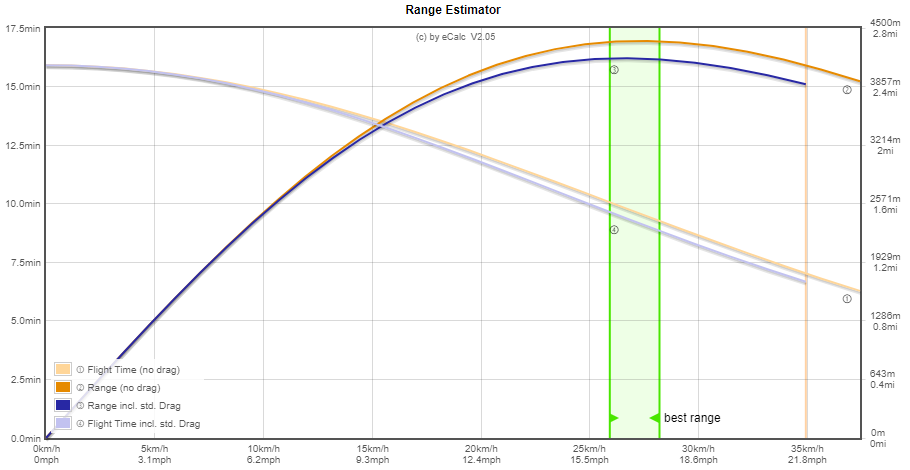
\includegraphics[width=0.75\textwidth]{powerGraph}
			\end{center}
		\end{figure}

		As for the 2000 [mAh] 3S battery, this battery powers our Pixhawk flight controller and our three Jetson TX2 compute units. This was done partly to dedicate the entirety of the main battery to propulsion to maximize flight time. The other reason is that the speed controllers we chose (T-motor Air 40A) have no BEC, so a separate battery for the flight controller (and in turn the receiver) was the simplest solution. 2000 [mAh] was chosen because of the slim form factor we were able to find it in, and because it will provide more than adequate power while not adding any significant amount to the quad weight.


\section*{Operations}
	\subsection*{Flight Preparations}
		\subsubsection*{Checklist}
			\begin{my_enumerate}
				\item Check battery voltage (12.0-12.6v) and insert
				\item Make sure LiDAR and PX4FLOW are not covered
				\item Make sure that ESCs are plugged in to the right pins
				\item Make sure prop guards are secure
				\item Make sure that the props are on in the correct direction (leading edge in)
				\item Make sure that the props are not upside down
				\item Make sure props are clear of any structures
				\item Make sure Kill Switch is in off position
				\item Power on controllers
				\item Make sure TELEM2 is unplugged
				\item Plug in power loop
				\item Turn Kill Switch to on position
				\item Make sure ground station has good telemetry
				\item Verify critical sensors are giving good data
				\item Plug in TELEM2
				\item SSH start/verify autonomous scripts are running
				\item Make sure everyone is clear of drone
				\item Verify mode switch in Stabilize
				\item Hold safety button
				\item Mode switch to Autonomous
			\end{my_enumerate}
	\subsection*{Man/Machine Interface}
		The drone has a DX7 RC controller interface for system checks and emergency situations. In addition, the flight controller can be monitored via a telemetry radio using Mission Planner. Our autonomous scripts must be initiated by an SSH connection to our Nvidia Jetsons.

\section*{Risk Reduction}
	\subsection*{Vehicle Status}
		\subsubsection*{Shock/Vibration Isolation}
		The modern Pixhawk flight controller contains internal damping from the vibration of the drone's structure. The team decided there is no need for extra damping. After completion of our first drone last year, flight logs from the Pixhawk confirmed that vibration on the built quadcopter was well within recommended amounts. The team believes there is no need to have landing shocks, because the sophisticated Arducopter flight stack has logic to recognize landing. Because of this, nominal landings will not interfere with the guidance or navigation of the drone.

		\subsubsection*{EMI/RFI Solutions}
		The Arducopter flight stack helps keep interference risk down through the EMI calibration on the Pixhawk. The calibration calculates the magnetic interference correction by formulating a function of the magnetic interference based on the power setting of the motors.


	\subsection*{Safety}
		We took significant steps to ensure safe operation of the quadcopter. In order to keep the quadcopter from flying where we do not want, we have a Spektrum receiver module onboard so our designated pilot can manually control the vehicle. Additionally, we are able to check the status of the quadcopter through our telemetry to our ground station. The structure of the drone is also outfitted with prop guards to mitigate damage to people or property in the event of catastrophic failure. Our prop guards took multiple iterations. We wanted a design that would not interfere with the prop wash, but still be able prevent damage to the quadcopter itself in the unfortunate event of collision. The first iteration looked nice, but interfered with the prop wash too much and weighed too much, reducing the thrust. However, the next iteration cut weight and did not interfere with the prop wash.


	\subsection*{Modeling and Simulation}

		To safely test our software throughout the development process, the team implemented a simulation using the Gazebo application. Using this tool, TAR was able to deploy full scale software in the loop simulation without jeopardizing hardware with each design iteration.

		To employ the Gazebo framework, the team imported a standard quadcopter model from the arducopter standard library and roomba models from Gazebo model library, which were then updated with the color coded plates and obstacle tubes prescribed for the competition. Additionally, the ground plain within the reproduction was changed to match the texture expected at the competition.

		Gazebo was chosen because of its compatibility with ROS and Ardupilot, the internal communication protocol employed onboard our drone. With this congruence, the exact same software run onboard the drone could be run within the simulation, complete with sensor feedback detected within the simulated instance. C++ scripts could then be utilized to enforce the correct roomba behaviors, scripting the robots using the same messaging environment as the quadcopter itself (ROS).

		Overall, modeling our software behavior within a Gazebo simulation greatly expedited the development process. By standardizing the simulation setup, tests could be conducted on multiple computers at any time, instead of requiring sluggish process of updating, calibrating, and flying the physical drone. Additionally, simulation protected the hardware from the accidents and unintentional flight behavior inherent to prototype software.


	\subsection*{Testing}
		Simulation, however, can only prove so much. Eventually, refined software was tested on a model testbed or on the drone itself. Much of the computer vision and general software integration was developed on this testbed, where performance could be verified with the same sensors and computational hardware as the aircraft before full scale deployment. Even strategy nodes could be tested on this platform, with waypoint predictions vetted before being deployed to the aircraft.

		Flight tests, expectedly, require a specific setting. Generally, Texas Aerial Robotics tested on the roof of the Aerospace building on campus at the The University of Texas. This controlled environment bore witness to hardware implementation throughout our design process, from original flight readiness to early autonomy.

		However, summer development saw additional test flights conducted in a vacant parking garage, but both locations suffered from magnetic inconsistencies which interfered with compass calibrations. Because of this, later tests, including the qualifying run submitted, were conducted in a parking lot to the north of the university.

		Regardless of the setting, each flight test was conducted with constant apparatus. A four meter by four meter test mat printed with the pattern expected at competition, to allow optical flow for navigation. Across this mat drives a test roomba, which accurately recreates both the physical appearance and behaviors of those robots that will be tracked at the venue, complete with top plate and switch. Finally, there is the drone itself, which starts on a corner of the mat, takes off autonomously, and then executes the maneuver to be tested.


\section*{Conclusion}
		Texas Aerial Robotics' solution to the challenges provided by IARC Mission 7 are bountiful and diverse. The physical design process, from the ground up, optimizes flight time while enabling the physical contact required for success, Unique software utilizes input from an expansive battery of sensors to overcome the telemetry limitations imparted by the contest and track the dynamic objectives as they move about the area. Safe operation of these vast networks of interlocking components has been ensured through particular hardware selection and thorough vetting.
	\nocite{redmon2016yolo9000}
	\nocite{GitHubSPACEROBOTICS}
	\nocite{HoughTransform}
	\nocite{CannyEdgeDetection}
	\bibliography{bibliography}
	\bibliographystyle{plain}

\end{document}
